Usein ollaan kiinnostuneita siitä, millainen yhteys on kahden asian välillä.
Funktio on matemaattinen työkalu näiden yhteyksien tarkastelemiseen.

\laatikko{ % tästä on jaksettu riidellä
	\termi{funktio}{Funktio} $f$ on sääntö, joka liittää \termi{muuttuja}{muuttujaan} $x$ arvon $f(x)$.

	Funktiolla on \termi{määrittelyjoukko}{määrittelyjoukko} $A$, johon muuttuja $x$ kuuluu,
	ja \termi{maalijoukko}{maalijoukko} $B$, johon funktion arvot kuuluvat.
}

\begin{esimerkki}
	Hyödykkeen ja siitä maksettavan arvonlisäveron välistä yhteyttä voidaan kuvata funktiolla.
	Valitaan funktion määrittelyjoukoksi tiettyjen hyödykkeiden joukko,
		\[ A = \{\text{ahvenfilee}, \text{AIV-rehu}, \text{auto}, \text{runokirja},
		\text{ravintola-ateria}, \text{särkylääke}, \text{televisio}\}, \]
	ja arvojoukoksi reaaliluvut.
	Funktio voi liittää kuhunkin hyödykkeeseen esimerkiksi siitä maksettavan arvonlisäveroprosentin:
	$f(\text{särkylääke}) = 10$ ja $f(\text{televisio}) = 24$.

	\begin{center}
		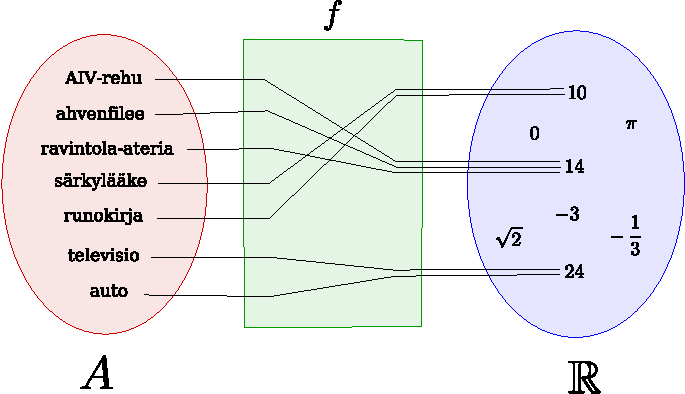
\includegraphics[width=11.5cm]{pictures/funktiokone.pdf}
	\end{center}
\end{esimerkki}

%\begin{esimerkki}
%Seuraavaan taulukkoon on koottu kuukausittaiset keskilämpötilat Sodankylässä vuonna 2012.
%	\begin{tabular}{|c|c|c|c|c|c|c|c|c|c|c|c|}
%	\hline
%	Tammi & Helmi & Maalis & Huhti & Touko & Kesä & Heinä & Elo & Syys & Loka & Marras & Joulu\\
%	\hline
%	-12 & -16 & -6 & -3 & 6 & 11 & 13 & 12 & 7 & 0 & -4 & -15\\
%	\hline
%	\end{tabular}
%Taulukon perusteella voidaan määritellä funktio \(f\) kuukausien joukolta lämpötilojen joukolle liittämällä jokaiseen kuukauteen sitä vastaava keskilämpötila. Silloin esimerkiksi \(f(Tammi)=-12\) ja \(f(Touko) = -3\). 
%%Lähtöjoukoksi mieluummin vain kuukausien järjestysnumerot? Lähde: Ilmatieteenlaitos
%\end{esimerkki}

Funktioiden merkitsemiseen liittyy joitakin vakiintuneita tapoja:
\begin{description}
	\item[1)] Merkintä $f(x) = y$ luetaan esimerkiksi: ''funktio \(f\) saa arvon $y$ pisteessä $x$'' tai lyhyemmin: ''\(f\) arvolla \(x\) on \(y\).''
	\item[2)] Funktion määrittely- ja maalijoukot jätetään usein merkitsemättä, jos ne voidaan päätellä asiayhteydestä.
		Tällä kurssilla funktiot ovat yleensä reaaliluvuilta reaaliluvuille.
	\item[3)] Usein kirjoitetaan esimerkiksi ''funktio $f(x) = x^2+3x$,'' vaikka tarkkaan ottaen funktio on $f$ ja
		$f(x)$ on sen saama arvo pisteessä $x$.
	\item[4)] Toisinaan funktiolle ja funktion kuvaajalle ei tehdä selkeää eroa:
		$y = f(x)$ samaistetaan koordinaatistoon piirretyn funktion kuvaajan kanssa.
		Oikeastaan funktio ja sen kuvaaja ovat kuitenkin eri asioita.
\end{description}
\begin{esimerkki}
Seuraava kuva esittää erään suotuisissa oloissa kehittyvän bakteerikannan massaa ajan \(t\) funktiona. 

\begin{kuva}
    kuvaaja.pohja(0, 8, 0, 8)
    kuvaaja.piirra("1.4**x", nimi = "$y=m(t)$")
\end{kuva}

Alkutilanteessa eli ajanhetkellä \(t=0\) bakteerikannan massa \(m(t)\) on \(m(0)=1\) gramma. Kahden tunnin kuluttua bakteerikannan massa on \(m(2)\approx 2,0\) grammaa ja kuuden tunnin kuluttua vastaavasti \(m(6)\approx 7,5\) grammaa. 
\end{esimerkki}

\subsection*{Reaalifunktiot}

Funktioita, jotka määritellään reaaliluvuilla, ja jotka saavat arvokseen reaalilukuja, kutsutaan reaalifunktioiksi.
Funktiolla, erityisesti reaalifunktioilla, on usein jokin selkeä sääntö, joka voidaan kirjoittaa matemaattisena lausekkeena.

\begin{esimerkki}
	Jos neliön sivun pituutta merkitään muuttujalla $x$, voidaan sivun pituuden
	ja neliön pinta-alan välistä yhteyttä kuvata funktiolla $A(x) = x^2$. % FIXME
\end{esimerkki}

Reaalifunktioita voidaan havainnollistaa koordinaatistossa kuvaajien avulla.
Funktion $f$ kuvaajassa koordinaatistoon piirretään ne pisteet $(x, y)$, joiden $y$-koordinaatti on $f$:n arvo $x$-koordinaatissa.
Reaalifunktioilla ei kuitenkaan voida laskea $y = f(x)$ kaikilla $f$:n määrittelyjoukon luvuilla $x$, joten esimerkiksi graafiset laskimet
laskevat $y = f(x)$ ''riittävän monella'' luvulla ja sovittavat kuvaajan niiden perusteella.
Funktioita voi piirtää helposti paitsi graafisilla laskimilla, myös tietokoneohjelmilla sekä esimerkiksi verkossa
Wolfram Alphalla (\url{http://www.wolframalpha.com/}).

% Tarvitaan kuvien ja taulukkojen vierekkäin laittamiseen.
\def\vcent#1{\mathsurround0pt$\vcenter{\hbox{#1}}$}

\begin{esimerkki}
	Funktion $f(x) = \frac{x}{2} - 1$ kuvaaja sisältää kaikki pisteet $(x, y)$, joilla pätee $y = \frac{x}{2} - 1$: % FIXME
	\begin{center}
		\begin{tabular}{cc}
			\begin{tabular}{|r|l|}
				\hline
				$x$ & $y = f(x)$ \\
				\hline
				$-3$ & $-2,5$ \\
				$-2$ & $-2$ \\
				$-1$ & $-1,5$ \\
				$0$ & $-1$ \\
				$1$ & $-0,5$ \\
				$2$ & $0$ \\
				$3$ & $0,5$ \\
				\hline
			\end{tabular} &
			\vcent{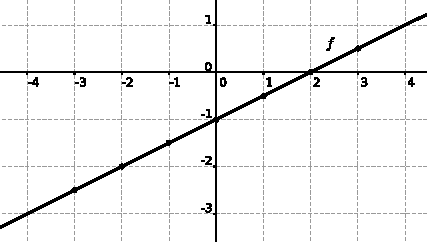
\includegraphics[width=8cm]{pictures/suoraesim.pdf}}
		\end{tabular}
	\end{center}
\end{esimerkki}

\begin{esimerkki}
	Funktion $f(x) = x^2$ kuvaaja sisältää kaikki pisteet $(x, y)$, joilla pätee $y = x^2$: % FIXME
	\begin{center}
		\begin{tabular}{cc}
			\begin{tabular}{|r|l|}
				\hline
				$x$ & $y = f(x)$ \\
				\hline
				$-2$ & $4$ \\
				$-1$ & $1$ \\
				$-0,5$ & $0.25$ \\
				$0$ & $0$ \\
				$0,5$ & $0.25$ \\
				$1$ & $1$ \\
				$2$ & $4$ \\
				\hline
			\end{tabular} &
			\vcent{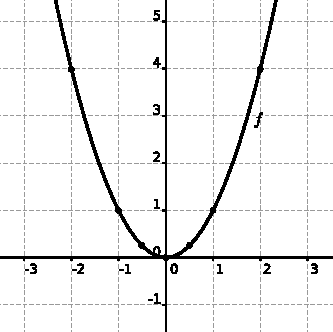
\includegraphics[width=6cm]{pictures/paraabeli.pdf}}
		\end{tabular}
	\end{center}
\end{esimerkki}

\begin{esimerkki}
	Funktion $f(x) = x^3-5x+2$ kuvaaja sisältää kaikki pisteet $(x, y)$, joilla pätee $y = x^3-5x+2$: % FIXME
	\begin{center}
		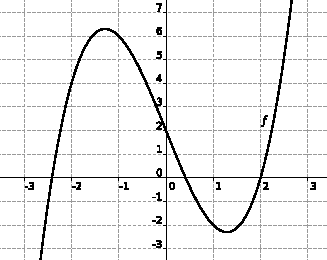
\includegraphics[width=7cm]{pictures/deg3polynomiesim.pdf}
	\end{center}
\end{esimerkki}

\subsection*{Määrittelyjoukko ja arvojoukko}

Funktion määrittelyjoukko koostuu niistä muuttujan arvoista, joilla
funktio on määritelty, eli joilla funktion arvo voidaan laskea.

\begin{esimerkki}
	Määritellään funktio $f$ lausekkeella \[ f(x) = \frac{1}{x-1}. \]
	Mikä on funktion määrittelyjoukko?
	\begin{esimratk}
		Funktio $f$ on määritelty, kun nimittäjä $x-1$ on erisuuri kuin 0.
		Tämä toteutuu kaikilla $x$:n arvoilla lukuun ottamatta arvoa $x = 1$.
		Funktion määrittelyjoukkoon kuuluvat siis kaikki reaaliluvut paitsi luku $1$.
	\end{esimratk}
	\begin{esimvast}
		Funktion $f$ määrittelyjoukko on reaalilukujen joukko poislukien luku $1$.
	\end{esimvast}
\end{esimerkki}

Funktion \termi{arvojoukko}{arvojoukko} sisältää ne maalijoukon alkiot,
jotka funktio saa arvokseen ainakin yhdessä pisteessä.

\begin{esimerkki}
	Mikä on edellä määritellyn funktion $f$ arvojoukko?
	% korjaa
	\begin{esimratk}
		Arvojoukon selvittämiseksi tutkitaan, millä luvun $a$ arvoilla
		yhtälöllä $f(x) = a$ on ratkaisu. Oletetaan, että $x \neq 1$ (ks. edellinen esimerkki).
		\begin{align*}
			a &= \frac{1}{x-1} & &| \, \cdot (x-1), \; \text{sillä} \; x \neq 1 \\
			a(x-1) &= 1
		\end{align*}
		Havaitaan, että jos $a = 0$, yhtälöllä ei voi olla ratkaisua, koska $0 \cdot (x-1) = 0 \neq 1$.
		Oletetaan jatkossa, että $a \neq 0$.
		\begin{align*}
			a(x-1) &= 1 & &| \, : a, \; \text{sillä} \; a \neq 0 \\
			x-1 &= \frac{1}{a} \\
			x &= 1+\frac{1}{a}
		\end{align*}
		Havaitaan, että yhtälöllä on ratkaisu kaikilla $a \neq 0$.
	\end{esimratk}
	\begin{esimvast}
		Funktion $f$ arvojoukko on reaalilukujen joukko poislukien luku $0$.
	\end{esimvast}
\end{esimerkki}
